\documentclass[11pt,a4paper]{article}
\usepackage[utf8]{inputenc}
\usepackage[spanish]{babel}
\usepackage{amsmath}
\usepackage{amsfonts}
\usepackage{amssymb}

\usepackage[hyphens]{url}
\usepackage{hyperref}

\usepackage{float}
\usepackage{graphicx}
\usepackage{geometry}
\usepackage{hyperref}
\usepackage{apacite}

\newgeometry{left=3cm, right=3cm, top=2.5cm, bottom=2.5cm}



\usepackage{listings}
\usepackage{xcolor}

\definecolor{codegreen}{rgb}{0,0.6,0}
\definecolor{codegray}{rgb}{0.5,0.5,0.5}
\definecolor{codepurple}{rgb}{0.58,0,0.82}
\definecolor{backcolour}{rgb}{0.95,0.95,0.92}

\lstdefinestyle{mystyle}{
	backgroundcolor=\color{backcolour},   
	commentstyle=\color{codegreen},
	keywordstyle=\color{magenta},
	numberstyle=\tiny\color{codegray},
	stringstyle=\color{codepurple},
	basicstyle=\ttfamily\footnotesize,
	breakatwhitespace=false,         
	breaklines=true,                 
	captionpos=b,                    
	keepspaces=true,                 
	numbers=left,                    
	numbersep=5pt,                  
	showspaces=false,                
	showstringspaces=false,
	showtabs=false,                  
	tabsize=2
}

\lstset{style=mystyle}



\begin{document}
\begin{titlepage}
\centering


{\bfseries\LARGE UNIVERSIDAD NACIONAL DEL ALTIPLANO\par}
{\scshape\LARGE Facultad de Ingeniería Mecánica Eléctrica, Electrónica y Sistemas\par}
{\scshape\LARGE Escuela Profesional de Ingeniería de Sistemas\par}
\vspace{1cm}
{
\includegraphics[width=0.6\textwidth]{images/1-unap.png}\par}
\vspace{0.5cm}
{\bfseries\LARGE Práctica N°2\par}
\vspace{1cm}
{\LARGE Docente: Mg. Aldo Hernan Zanabria Galvez \par}

{\LARGE Alumno: Yoel Nhelio Canaza Chagua \par}
\vspace{1cm}
{\LARGE Curso: \par}
{\LARGE Programación Orientada a Objetos II \par}
\vspace{1cm}
{\LARGE CICLO III – SEMESTRE 2023 – II \par}
{\LARGE PUNO, PERÚ \par}
{\LARGE 2023 \par}


\end{titlepage}

\section{Objetivos}
\begin{enumerate}
    \item Creación de Clases y Objetos: Practicar la creación de clases (Libro y Biblioteca) y la instanciación de objetos a partir de esas clases.
    \item Atributos y Métodos: Entender cómo definir atributos (como titulo, autor, anio\_publicacion, y disponible) y métodos en una clase.
    \item Encapsulación: Aplicar el concepto de encapsulación al usar atributos privados y proporcionar métodos públicos para interactuar con esos atributos.
    \item Operaciones Básicas: Realizar operaciones básicas sobre los objetos, como agregar un libro a la biblioteca, buscar un libro por título, prestar un libro y devolver un libro.
    \item Manejo de Listas: Trabajar con listas para mantener un conjunto de libros en la biblioteca.
    \item Mensaje de Usuario: Incluir mensajes informativos para el usuario, como confirmaciones de acciones realizadas.

\end{enumerate}

\section{Desarrollo}

\begin{lstlisting}[language=Python, style=mystyle, caption={Código base sin modificaciones.}]
class Libro:
    def __init__(self, titulo, autor, anio_publicacion):
        self.titulo = titulo
        self.autor = autor
        self.anio_publicacion = anio_publicacion
        self.disponible = True

    def __str__(self):
        disponibilidad = "disponible" if self.disponible else "prestado"
        return f"{self.titulo} - {self.autor} ({self.anio_publicacion}), {disponibilidad}"

class Biblioteca:
    def __init__(self):
        self.libros = []

    def agregar_libro(self, libro):
        self.libros.append(libro)
        print(f"Libro '{libro.titulo}' agregado a la biblioteca.")

    def buscar_libro(self, titulo):
        for libro in self.libros:
            if libro.titulo == titulo:
                return libro
        return None

    def prestar_libro(self, titulo):
        libro = self.buscar_libro(titulo)
        if libro:
            if libro.disponible:
                libro.disponible = False
                print(f"Libro '{libro.titulo}' prestado.")
            else:
                print(f"El libro '{libro.titulo}' no está disponible en este momento.")
        else:
            print(f"No se encontró el libro con título '{titulo}' en la biblioteca.")

    def devolver_libro(self, titulo):
        libro = self.buscar_libro(titulo)
        if libro:
            if not libro.disponible:
                libro.disponible = True
                print(f"Libro '{libro.titulo}' devuelto.")
            else:
                print(f"El libro '{libro.titulo}' ya está disponible en la biblioteca.")
        else:
            print(f"No se encontró el libro con título '{titulo}' en la biblioteca.")

# Crear algunos libros
libro1 = Libro("Python Crash Course", "Eric Matthes", 2015)
libro2 = Libro("Clean Code", "Robert C. Martin", 2008)
libro3 = Libro("The Art of Computer Programming", "Donald E. Knuth", 1968)

# Crear una biblioteca
biblioteca = Biblioteca()

# Agregar libros a la biblioteca
biblioteca.agregar_libro(libro1)
biblioteca.agregar_libro(libro2)
biblioteca.agregar_libro(libro3)

# Realizar operaciones de préstamo y devolución
biblioteca.prestar_libro("Clean Code")
biblioteca.devolver_libro("Python Crash Course")
biblioteca.prestar_libro("The Art of Computer Programming")

# Mostrar información de los libros en la biblioteca
print("\nEstado actual de la biblioteca:")
for libro in biblioteca.libros:
    print(libro)

\end{lstlisting}


\section{Problema}
Crea una clase llamada Libro que tenga los siguientes atributos:

\begin{itemize}
    \item titulo (cadena): el título del libro.
    \item autor (cadena): el autor del libro.
    \item anio\_publicacion (entero): el año de publicación del libro.
    \item disponible (booleano): indica si el libro está disponible para ser prestado.
    \item Luego, crea una clase llamada Biblioteca que tenga una lista de libros y los siguientes métodos:
\begin{itemize}
    \item agregar\_libro(libro): agrega un libro a la biblioteca.
    \item buscar\_libro(titulo): busca un libro por su título y devuelve la información del libro si está en la biblioteca.
    \item prestar\_libro(titulo): marca un libro como prestado si está disponible.
    \item devolver\_libro(titulo): marca un libro como disponible si estaba prestado.
\end{itemize}
\end{itemize}

\section{Ejercicios Planteados}
El código con las modificaciones guardado en:
\begin{sloppypar}
\url{https://github.com/YoelCanaza/poo2-practica-2/blob/2289090a20512564e76f267bf34728590dbd6293/practica-2.py}
\end{sloppypar}

\lstinputlisting[language=Python, style=mystyle, caption={Código con todas las modificaciones pedidas en los ejercicios}]{practica-2.py}

\begin{figure}[H]
    \centering
    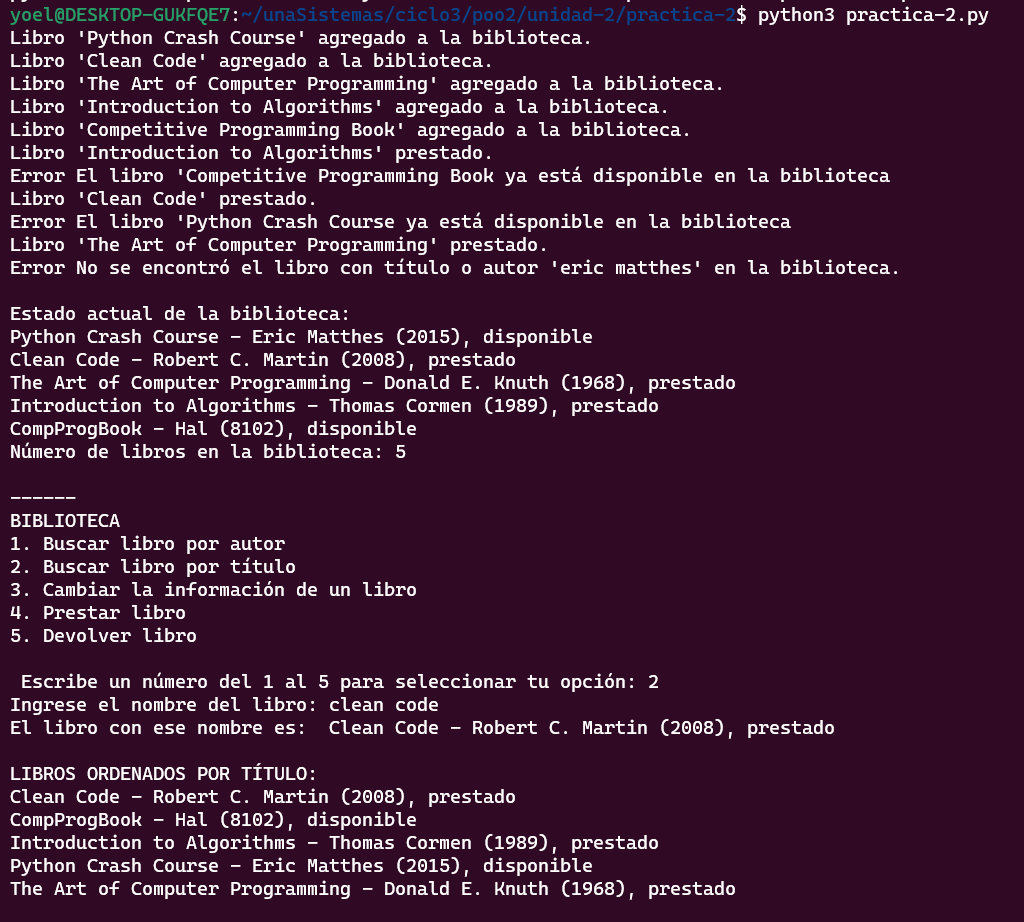
\includegraphics[width=1\linewidth]{images/compilado.png}
    \caption{}
    \label{fig:enter-label}
\end{figure}

\begin{figure}[H]
    \centering
    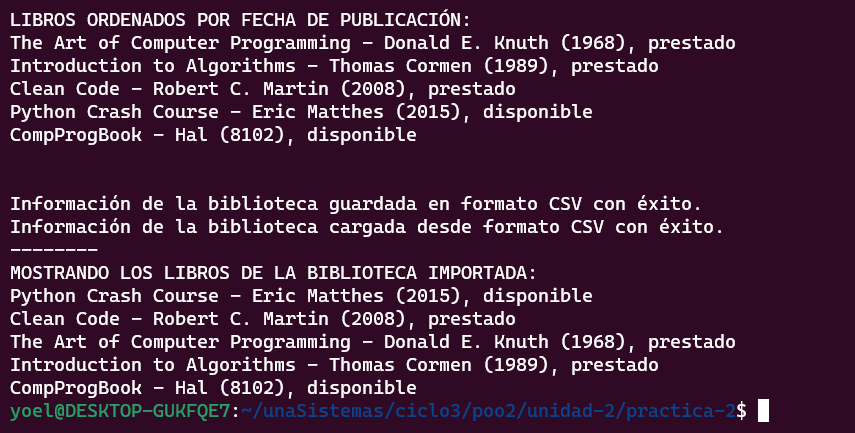
\includegraphics[width=0.8\linewidth]{images/compilado-2.png}
    \caption{}
    \label{fig:enter-label}
\end{figure}

\subsection{Agregar más libros:
Modifica el código para agregar al menos dos libros más a la biblioteca.
Realiza operaciones de préstamo y devolución con estos nuevos libros.}

\begin{figure}[H]
    \centering
    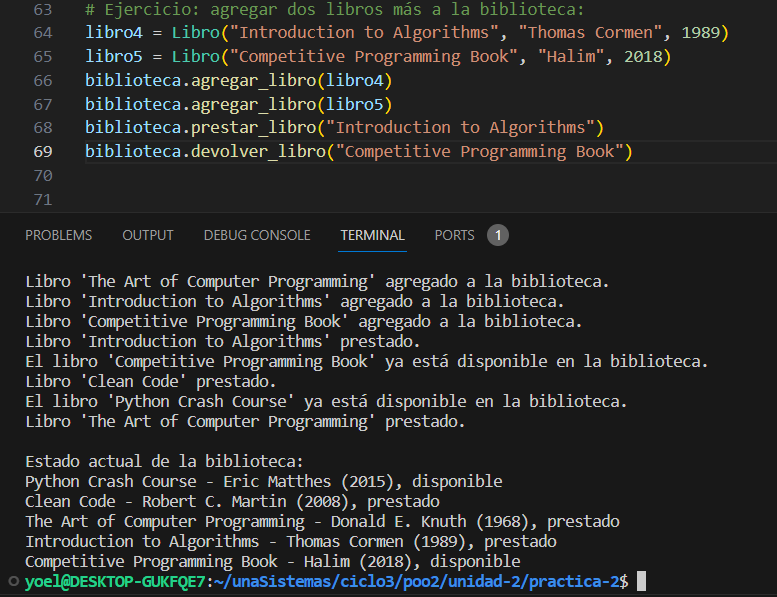
\includegraphics{images/2-ejercicio1.png}
    \caption{Caption}
    \label{fig:enter-label}
\end{figure}

\subsection{Mejorar la búsqueda:
Modifica el método buscar\_libro para que sea insensible a mayúsculas/minúsculas al buscar por título.
Implementa una búsqueda que permita encontrar libros por autor.}
\begin{figure}[H]
    \centering
    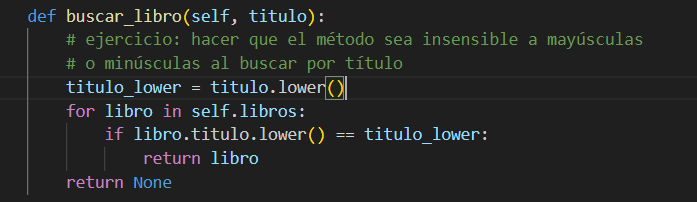
\includegraphics{images/3-ej2-1.png}
    \caption{Método modificado para que sea insensible a mayúsculas/minúsculas}
    \label{fig:enter-label}
\end{figure}

\begin{figure}[H]
    \centering
    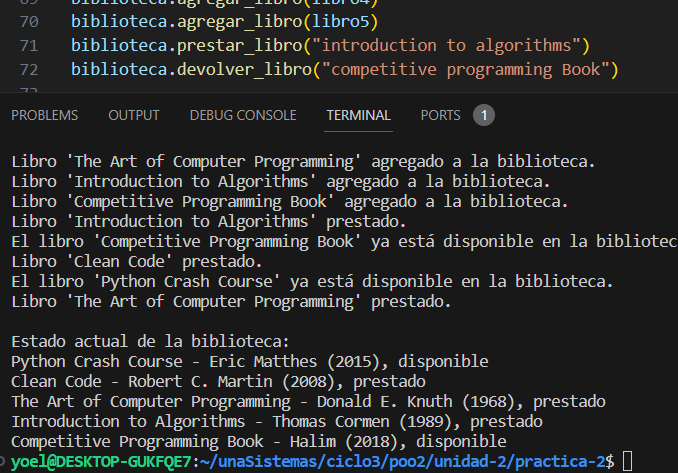
\includegraphics{images/3-ej2-2.png}
    \caption{Gracias a la función modificada, se puede poner como argumentos los títulos de los libros en minúsculas}
    \label{fig:enter-label}
\end{figure}
\subsubsection{búsqueda por autor}
\begin{figure}[H]
    \centering
    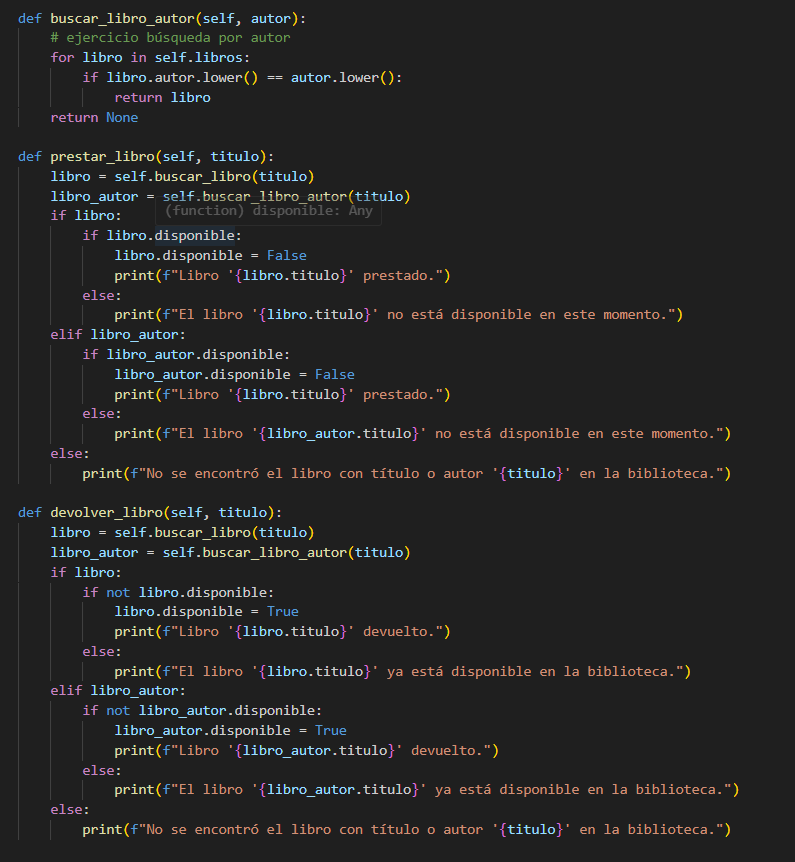
\includegraphics[width=0.7\textwidth] {images/3-eje2-3.png}
    \caption{También se modificaronlas funciones prestar libro y devolver libro para que se pueda poner como argumento autor o nombre del libro}
    \label{fig:enter-label}
\end{figure}

\begin{figure}[H]
    \centering
    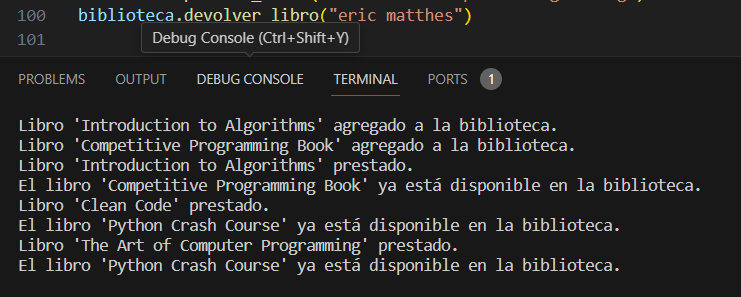
\includegraphics{images/3-eje2-4.png}
    \caption{Como se puede ver en la imagen, como argumento de la función devolver libro se puso el nombre del autor y en minúsculas. Gracias a las modificaciones, la operación se pudo realizar sin problemas}
    \label{fig:enter-label}
\end{figure}

\subsection{Conteo de libros:
Agrega un método a la clase Biblioteca que cuente y muestre la cantidad total de libros en la biblioteca.
Modifica la salida para incluir esta información.}

\begin{figure}[H]
    \centering
    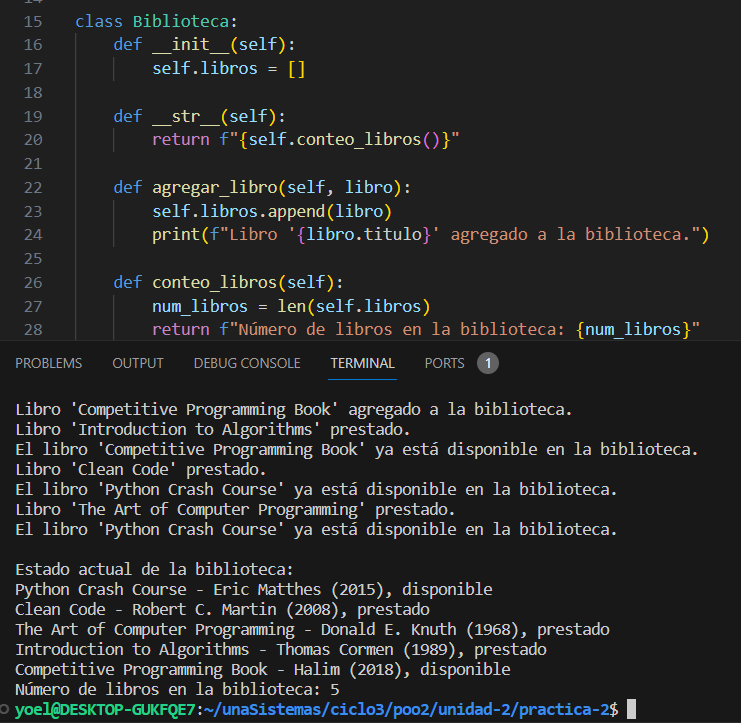
\includegraphics[width=0.9\textwidth]{images/4-ej3.png}
    \caption {Método para contar y mostrar los libros de la biblioteca}
    \label{fig:enter-label}
\end{figure}

\subsection{Actualizar información:
Agrega un método a la clase Libro que permita actualizar la información de un libro (título, autor, año de publicación).
Utiliza este método para actualizar la información de al menos un libro en la biblioteca.}
\begin{figure}[H]
    \centering
    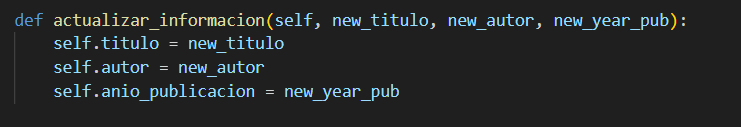
\includegraphics[width=1\linewidth]{images/5.png}
    \caption{Método en la claes libro para actualizar información}
    \label{fig:enter-label}
\end{figure}

\begin{figure}[H]
    \centering
    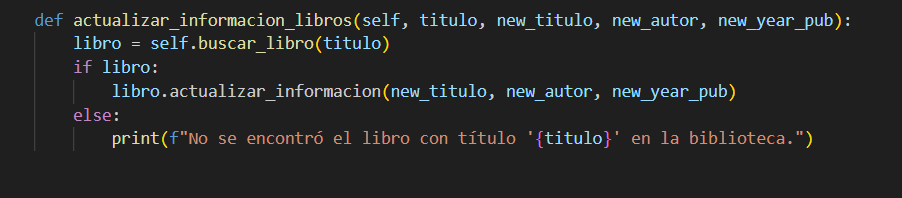
\includegraphics[width=1\linewidth]{images/5-2.png}
    \caption{Método miembro de Biblioteca pra buscar un libro y actualizar su información}
    \label{fig:enter-label}
\end{figure}

\begin{figure}[H]
    \centering
    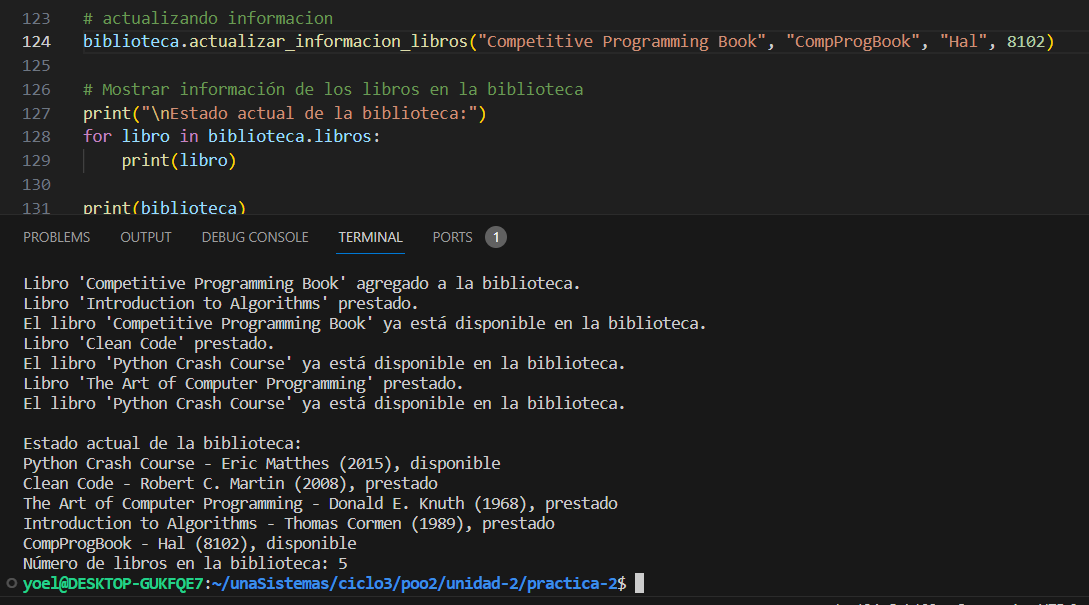
\includegraphics[width=1\linewidth]{images/5-3.png}
    \caption{Utilización del método para actualizar la información de un libro}
    \label{fig:enter-label}
\end{figure}

\subsection{Validaciones adicionales:
Mejora el código para incluir validaciones adicionales, como asegurarse de que el año de publicación sea un número positivo.}

\begin{figure}[H]
    \centering
    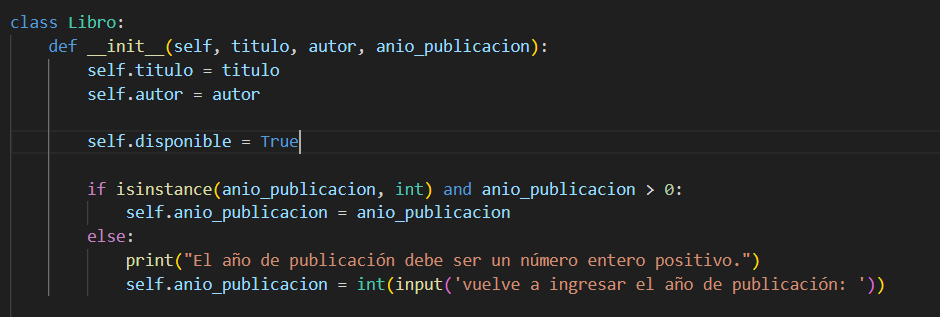
\includegraphics[width=1\linewidth]{images/6-validacion.png}
    \caption{Se valida que el año de publicación sea un entero positivo}
    \label{fig:enter-label}
\end{figure}

\subsection{Interfaz de usuario mejorada:
Crea una interfaz de usuario simple en la consola para que el usuario pueda interactuar con la biblioteca (por ejemplo, seleccionar opciones desde un menú).}

\begin{figure}[H]
    \centering
    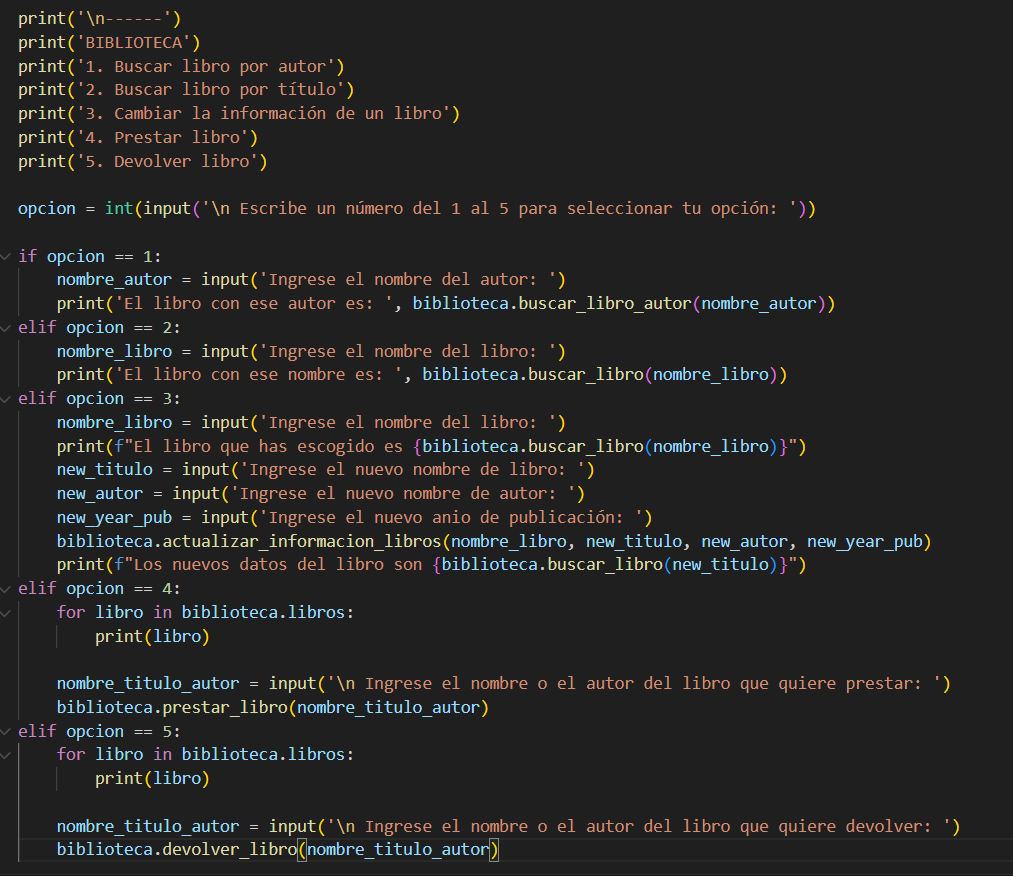
\includegraphics[width=1\linewidth]{images/7-codigo.png}
    \caption{}
    \label{fig:enter-label}
\end{figure}

\begin{figure}[H]
    \centering
    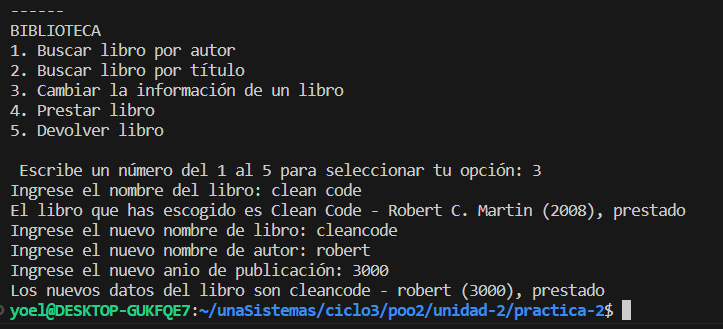
\includegraphics[width=0.8\linewidth]{images/7-comp.png}
    \caption{}
    \label{fig:enter-label}
\end{figure}
	
\subsection{Manejo de excepciones:
Implementa manejo de excepciones para situaciones como buscar un libro que no está en la biblioteca o devolver un libro que ya está disponible.}

\begin{figure}[H]
    \centering
    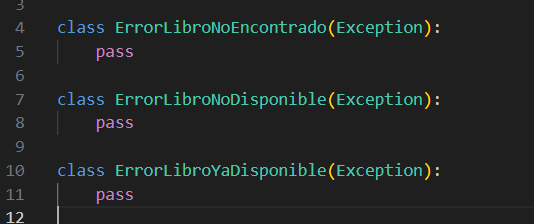
\includegraphics[width=0.5\linewidth]{images/8-1.png}
    \caption{Creamos nuevas clases de excepciones que heredan de 'Exception'}
    \label{fig:enter-label}
\end{figure}

\begin{figure}[H]
    \centering
    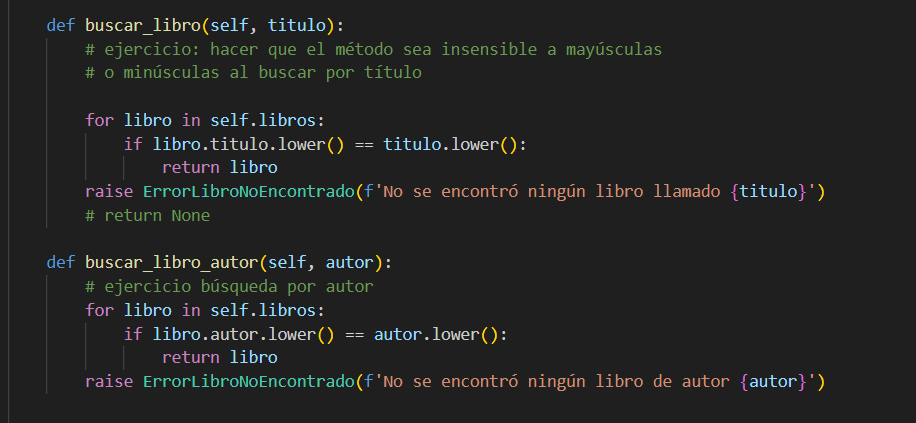
\includegraphics[width=1\linewidth]{images/8-2.png}
    \caption{Las funciones de búsqueda por título y búsqueda por autor se modifican para lanzar excepciones en caso de que no se encuentre el libro en la biblioteca}
    \label{fig:enter-label}
\end{figure}

\begin{figure}[h]
    \centering
    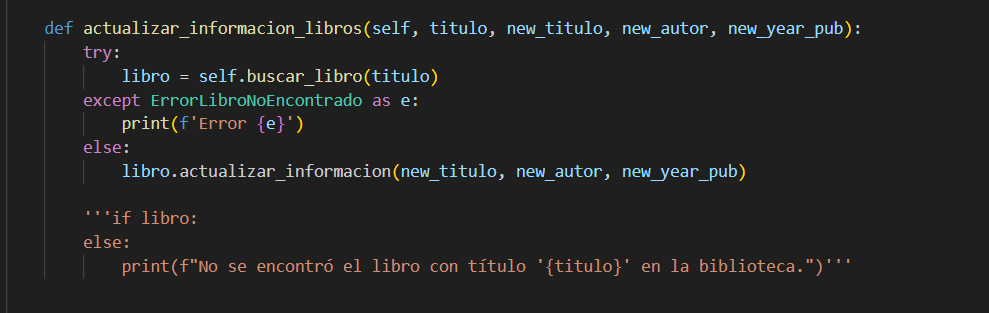
\includegraphics[width=1\linewidth]{images/8-3.png}
    \caption{La función para actualizar información de los libros también se modifica para lanzar y atrapar la excepción ErrorLibroNoEncontrado.}
    \label{fig:enter-label}
\end{figure}


\begin{figure}[H]
    \centering
    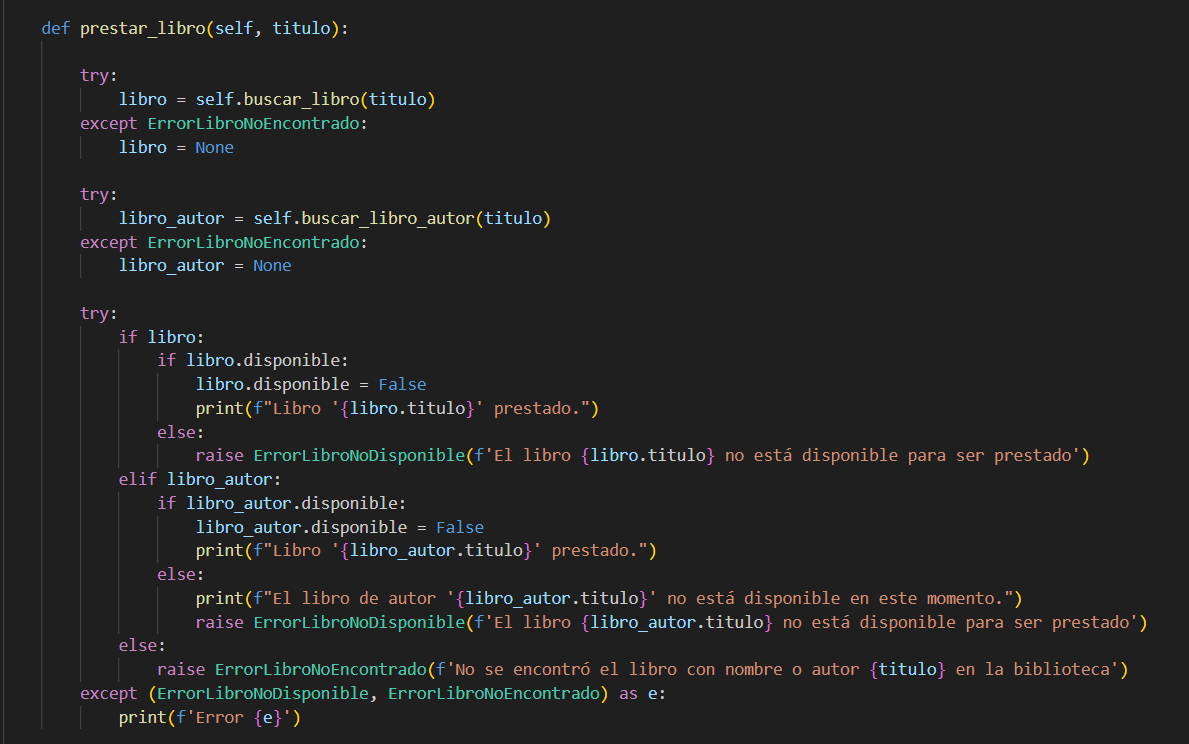
\includegraphics[width=1\linewidth]{images/8-4.png}
    \caption{Manejo de excepciones en caso de que se intente tomar prestado un libro que no se encuentra disponible}
    \label{fig:enter-label}
\end{figure}


\begin{figure}[H]
    \centering
    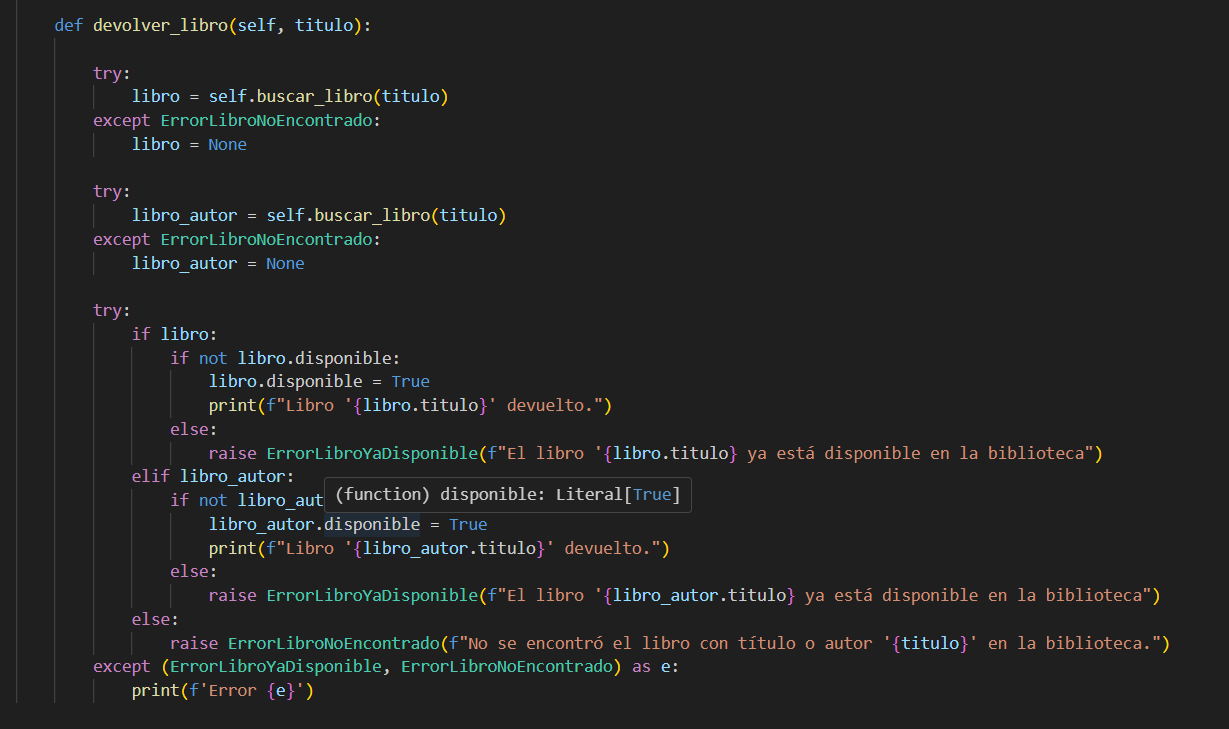
\includegraphics[width=1\linewidth]{images/8-5.png}
    \caption{Manejo de excepciones en caso de que se intente devolver un libro que ya está disponible}
    \label{fig:enter-label}
\end{figure}

\subsection{Ordenar libros:
Agrega un método a la clase Biblioteca que permita ordenar los libros por título o por año de publicación.
Muestra la lista ordenada de libros en la biblioteca.}


\begin{figure}[H]
    \centering
    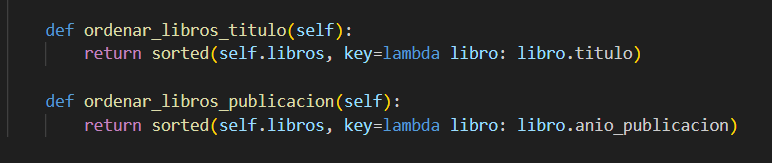
\includegraphics[width=1\linewidth]{images/9-1.png}
    \caption{Métodos para ordenar los libros por título o por año de publicación}
    \label{fig:enter-label}
\end{figure}


\begin{figure}[H]
    \centering
    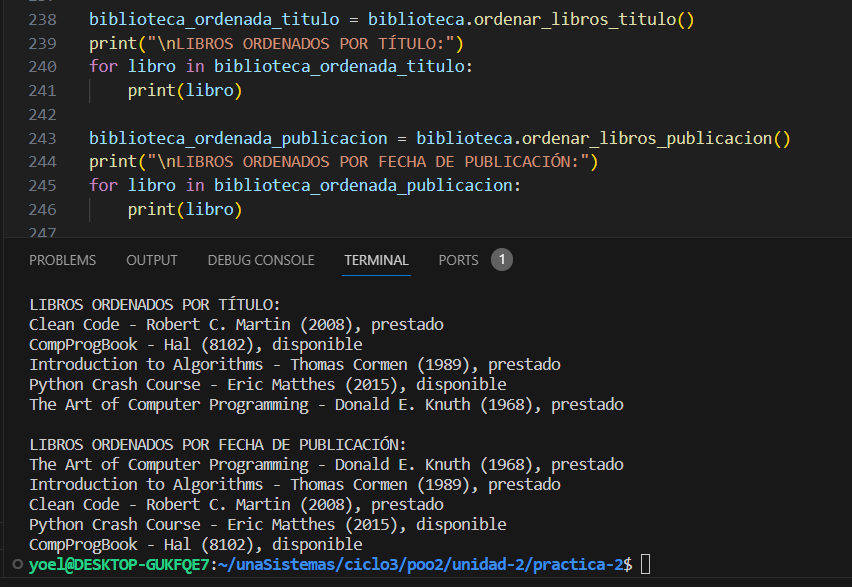
\includegraphics[width=1\linewidth]{images/9-2.png}
    \caption{Mostrando las listas ordenadas por título y por año de publicación}
    \label{fig:enter-label}
\end{figure}

\subsection{Guardar y cargar datos:
Agrega métodos a la clase Biblioteca para guardar y cargar la información de la biblioteca desde y hacia un archivo, respectivamente.}

\begin{figure}[H]
    \centering
    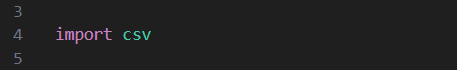
\includegraphics[width=0.5\linewidth]{images/10-1.png}
    \caption{IMportamos la librería CSV par poder para poder guardar y cargar información en archivos .csv}
    \label{fig:enter-label}
\end{figure}

\begin{figure}[H]
    \centering
    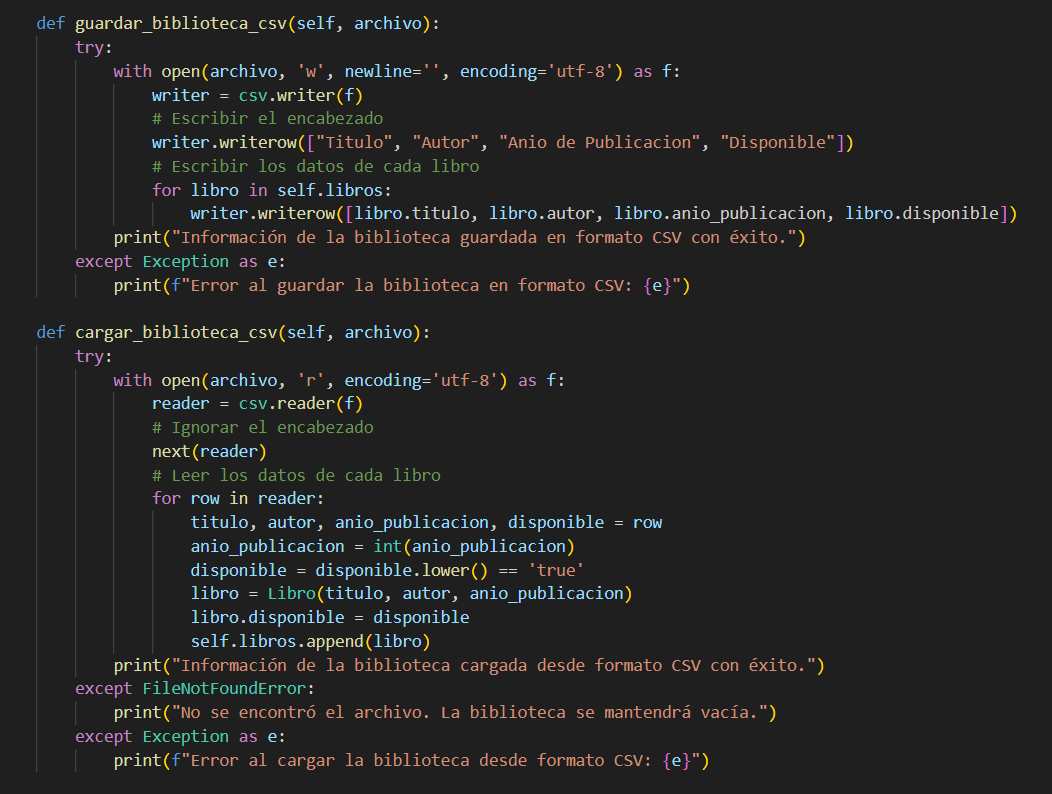
\includegraphics[width=0.8\linewidth]{images/10-2.png}
    \caption{Métodos para guardar y cargar la información de la biblioteca desde y hacia un archivo .csv}
    \label{fig:enter-label}
\end{figure}

\begin{figure}[H]
    \centering
    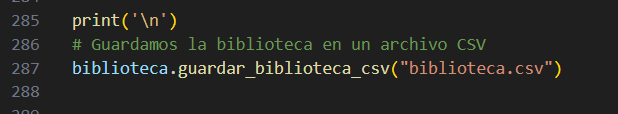
\includegraphics[width=1\linewidth]{images/10-3.png}
    \caption{Uso del método guardar_biblioteca_csv dentro del programa}
    \label{fig:enter-label}
\end{figure}

\begin{figure}[H]
    \centering
    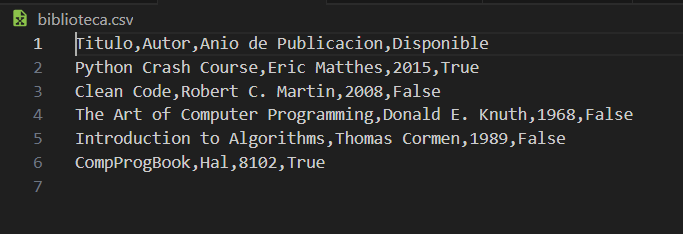
\includegraphics[width=1\linewidth]{images/10-4.png}
    \caption{Archivo .csv con la información de la biblioteca dentro}
    \label{fig:enter-label}
\end{figure}


\begin{figure}[H]
    \centering
    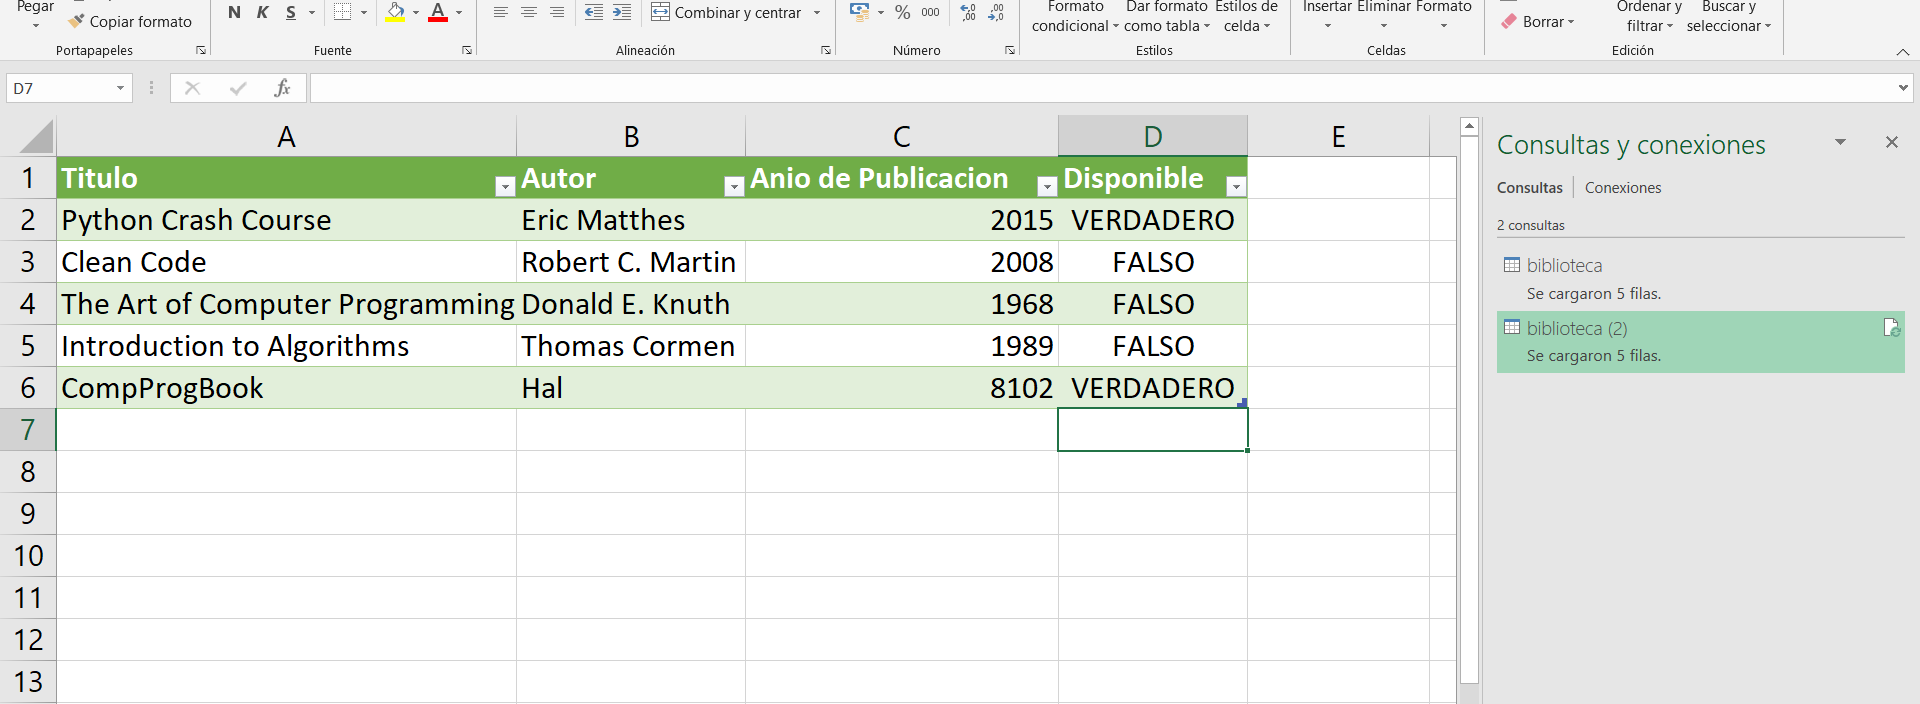
\includegraphics[width=1\linewidth]{images/10-5.png}
    \caption{Archivo .csv abierto con el programa 'Excel'}
    \label{fig:enter-label}
\end{figure}

\begin{figure}[H]
    \centering
    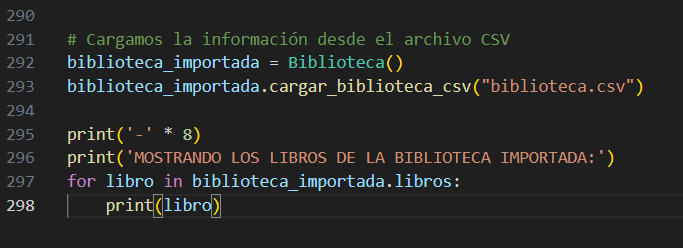
\includegraphics[width=1\linewidth]{images/10-6.png}
    \caption{Creando una nueva biblioteca para asignarle los datos desde el .csv}
    \label{fig:enter-label}
\end{figure}

\begin{figure}[H]
    \centering
    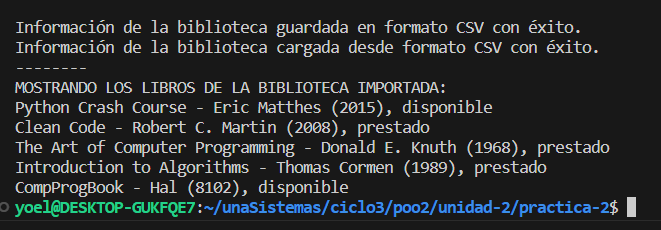
\includegraphics[width=1\linewidth]{images/10-7.png}
    \caption{}
    \label{fig:enter-label}
\end{figure}


\end{document}